%% Exemple de source LaTeX pour un article soumis à CORIA-TALN 2026
\documentclass[10pt,twoside]{article}

\usepackage{times}
\usepackage[utf8]{inputenc}
\usepackage[T1]{fontenc}
\usepackage{graphicx}
\usepackage{booktabs}
\usepackage{float} % option [H] pour figurer les figures à l'emplacement du code
\usepackage{amssymb} % pour \checkmark dans les tableaux

% Faire les \usepackage dont vous avez besoin de préférence AVANT le \usepackage{coria-taln2025}

% coria-taln2025 charge le package hyperref. Pour des raisons de compatibilités, certains
% package doivent donc néanmoins être chargés après le \usepackage{jeptaln2020}, comme
% par exemple le package linguex (voir les compatibilités sur http://distrib-coffee.ipsl.jussieu.fr/pub/mirrors/ctan/macros/latex/contrib/hyperref/doc/manual.html#x1-520009)

% Merci de *NE PAS* modifier la géométrie (les marges) ni les fontes
% et le caractère (10pt, times)

% Pour éviter l'espace après les virgules dans le mode math
\usepackage{siunitx}
\sisetup{locale = FR}
%\sisetup{output-decimal-marker = {,}}

% Load hyperref near the end
\usepackage{hyperref}
% Optional: cleveref after hyperref, if you use it
\usepackage{cleveref}
\usepackage{coria-taln2026}
\usepackage[french]{babel} %frenchb deprecated, use french instead

% Titre complet
\title{Affinage de modèles génératifs pour l'inférence en langue naturelle pour les essais cliniques : XXXX et YYYYY}

\author{Prénom1 Nom1\up{1, 2}\quad Prénom2 Nom2\up{1, 3}\\
  {\small
    Université-Paris-Saclay, CNRS, Laboratoire Interdisciplinaire des Sciences du Numérique
    \texttt{
      utrucmuche@lab.fr, umachinchose@adresse-academique.be \\ 
}}}

\begin{document}
% Références \ref{} : compiler au moins 2 fois (ou lancer ./compile_pdf.sh). Dans Cursor/VSCode, utiliser la recette « pdflatex x2 » de LaTeX Workshop.
\maketitle

\resume{
  Les Grands Modèles de Langage ont démontré des résultats compétitifs pour de nombreuses applications, y compris dans des domaines de spécialité comme le domaine biomédical. 
}

\abstract{Here the title in English.}{
  Here an abstract in English (max. 150 words).
}

\motsClefs
  {Inférence en langue naturelle, Grands Modèles de Langage, essais cliniques, affinage, apprentissage avec peu d'exemples}
  {Natural language inference, Large Language Models, clinical trials, finetuning, few-shot learning}

%---------------------------------------------------------------------------------------------------------------------
%%%% IMPORTANT ! %%%%
% Si votre article est une contribution originale alors COMMENTER les instructions \acceptedArticle[]{}{}


%---------------------------------------------------------------------------------------------------------------------
\section{Introduction}





%%================================================================
\section{Travaux connexes}

Ici on met les travaux précédemment publiés dans la littérature. 



%%================================================================

\section{Méthodes}

\subsection{Préparation des données NLI4PR}
Notre jeu de données présente (NLI4PR) une spécificité majeure : pour chaque patient, nous disposons de deux descriptions équivalentes sur le plan clinique, mais formulées différemment. La première est rédigée dans un langage médical technique (destiné aux professionnels), tandis que la seconde est formulée dans un langage courant (langage patient). 

Afin d'optimiser les temps de calcul et de s'adapter aux contraintes de ressources matérielles, la phase de \textit{fine-tuning} n'a pas été réalisée sur l'intégralité des données. Nous avons opté pour un échantillonnage aléatoire consistant à extraire 50\,\% du jeu d'entraînement rédigé en langage médical et 50\,\% de celui en langage patient. Ces deux sous-ensembles ont ensuite été fusionnés et mélangés aléatoirement (\textit{seed} fixée à 42 pour la reproductibilité) afin d'exposer le modèle aux deux registres de vocabulaire lors de son apprentissage. La phase d'évaluation finale a, quant à elle, été menée de manière exhaustive sur les deux ensembles de test séparément, permettant ainsi une analyse comparative détaillée des performances selon le type de langage.

\subsection{Structure et stratégies de Prompting NLI4PR}
Pour interroger le modèle, trois stratégies de formatage des requêtes (\textit{prompts}) ont été mises en œuvre et comparées :
\begin{itemize}
    \item \textbf{Standard NLI Prompt :} Cette approche classique de \textit{Natural Language Inference} (NLI) sépare le texte en deux blocs distincts : une \texttt{Premise} (contenant les critères d'inclusion et d'exclusion de l'essai) et une \texttt{Hypothesis} (contenant la description du patient). Le modèle reçoit pour instruction système stricte de classer la relation en répondant uniquement par « Entailment » (Éligible) ou « Contradiction » (Non-éligible).
    \item \textbf{Clinical Matching :} Cette stratégie reformule la tâche NLI sous la forme d'une question clinique directe et naturelle. Le prompt est structuré ainsi : \textit{« Does the patient with the statement [Description du patient] satisfy the following clinical trial admission criteria? [Critères] »}. L'instruction impose toujours une réponse en un seul mot.
    \item \textbf{Chain of Thought (CoT) Prompt :} Reposant sur la même structure que le Clinical Matching, cette approche intègre une consigne poussant le modèle à expliciter son raisonnement avant de conclure. L'instruction ajoutée est la suivante : \textit{« First, explain your reasoning step-by-step by comparing the patient's characteristics to the inclusion and exclusion criteria. Then, conclude on a new line with only one word: 'Entailment' or 'Contradiction' »}.
\end{itemize}

\subsection{Configuration du modèle et Fine-tuning (NLI4PR et NLI4CT)}
Le modèle de base sélectionné pour nos expériences est \textbf{Qwen 2.5 7B Instruct} (\texttt{Qwen2.5-7B-Instruct}), reconnu pour ses excellentes capacités de raisonnement et de suivi d'instructions. Cette même configuration est utilisée pour les deux jeux de données (NLI4PR et NLI4CT).

Pour rendre l'entraînement réalisable efficacement, nous avons appliqué une méthode d'optimisation paramétrique efficace (PEFT) basée sur \textbf{LoRA} (Low-Rank Adaptation). Les hyperparamètres LoRA ont été configurés avec un rang $r=16$, un \textit{alpha} de 32, et un \textit{dropout} de 0.05. L'adaptation a été ciblée sur l'ensemble des modules de projection de l'architecture \textit{Transformer} (\texttt{q\_proj}, \texttt{k\_proj}, \texttt{v\_proj}, \texttt{o\_proj}, \texttt{gate\_proj}, \texttt{up\_proj}, \texttt{down\_proj}). De plus, le modèle de base a été quantifié en 4-bit via \texttt{bitsandbytes} (format \textit{nf4} avec double quantification) pour réduire l'empreinte mémoire, en utilisant la précision \texttt{bfloat16} pour les calculs.

L'entraînement a été réalisé à l'aide de la bibliothèque \texttt{trl} (\textit{SFTTrainer}). Pour NLI4PR, le nombre d'époques a été fixé à 4 afin de limiter le temps de calcul~; pour NLI4CT, l'affinage a été conduit sur 5 époques. La taille de lot (\textit{batch size}) a été fixée à 2 par dispositif avec 4 étapes d'accumulation de gradient (\textit{gradient accumulation steps}). Le taux d'apprentissage (\textit{learning rate}) était de $2 \times 10^{-4}$. La longueur maximale de séquence a été fixée à 4096 \textit{tokens} afin d'éviter toute troncature des descriptions cliniques les plus longues, et le \textit{gradient checkpointing} a été activé pour optimiser l'usage de la mémoire.

\subsection{Stratégies d'Évaluation et Inférence NLI4PR}
Pour garantir la robustesse des métriques d'évaluation (\textit{Accuracy}, \textit{F1-score}), des stratégies de traitement des réponses (\textit{parsing}) spécifiques ont été développées selon la stratégie de \textit{prompting} utilisée. Lors de toutes les inférences, la température a été fixée à 0.7 avec un \textit{top-p} de 1.0.

\paragraph{Évaluation des prompts NLI et Clinical Matching NLI4PR}
Dans ces configurations, le modèle est instruit pour répondre par un mot unique. Par conséquent, la génération a été bridée à un maximum de 10 \textit{tokens} (\texttt{max\_new\_tokens=10}). Bien que la consigne soit stricte, les LLMs peuvent occasionnellement générer des espaces initiaux ou des signes de ponctuation. Notre algorithme d'évaluation convertit la réponse en minuscules et recherche la présence des racines \texttt{entail} ou \texttt{contradict} dans les 50 premiers caractères générés. Si les mots-clés sont identifiés, la prédiction est catégorisée en conséquence ; sinon, le texte brut est retourné pour vérification manuelle.

\paragraph{Évaluation du prompt Chain of Thought (CoT) NLI4PR}
Contrairement aux approches précédentes, le modèle génère ici un texte explicatif complet. La limite de génération a donc été étendue à 1024 \textit{tokens} (\texttt{max\_new\_tokens=1024}). Le mot-clé déterminant la prédiction se trouvant à la fin du raisonnement, la méthode d'extraction employée découpe la réponse générée par sauts de ligne, isole la dernière ligne non vide, et y recherche les mots-clés de classification. En cas d'absence de saut de ligne (non-respect occasionnel de la consigne), une méthode de secours inspecte l'intégralité du texte. Cette approche garantit une classification automatisée fiable tout en conservant le texte du raisonnement pour une analyse ultérieure.

\subsection{Préparation des données NLI4CT}
Le jeu de données NLI4CT (\textit{Natural Language Inference for Clinical Trials}) repose sur des protocoles d'essais cliniques : pour chaque instance, une \textbf{prémisse} est constituée par l'extraction de critères ou d'informations depuis des sections structurées des protocoles (Eligibility, Intervention, Adverse Events, etc.), et une \textbf{hypothèse} (\textit{Statement}) décrit une affirmation à évaluer au regard de cette prémisse. Le label est binaire : \texttt{Entailment} (l'affirmation est supportée par les critères) ou \texttt{Contradiction}. Deux types de tâches sont représentés : \textbf{Single} (un seul essai de référence) et \textbf{Comparison} (comparaison entre un essai primaire et un essai secondaire), ce qui permet d'évaluer à la fois l'éligibilité simple et le raisonnement comparatif. Les données sont issues des fichiers \texttt{train.json}, \texttt{dev.json} et d'un ensemble \texttt{Gold\_test.json} (500 exemples) utilisé pour l'évaluation finale. Les preuves sont extraites depuis des fichiers JSON par essai (\texttt{CT\_json}) en fonction des indices de preuve associés à chaque entrée.

\subsection{Structure et stratégies de Prompting NLI4CT}
Pour NLI4CT, deux formats de prompt ont été comparés, en cohérence avec une formulation NLI classique prémisse/hypothèse :
\begin{itemize}
    \item \textbf{Prompt 1 (NLI standard) :} Le message système demande de classer la relation entre la prémisse et l'hypothèse en répondant par un seul mot (\texttt{Entailment} ou \texttt{Contradiction}). Le contenu utilisateur est structuré en deux blocs : \texttt{PREMISE:} (contenant les critères ou extraits de protocole) et \texttt{HYPOTHESIS:} (l'énoncé à évaluer).
    \item \textbf{Prompt 2 (question explicite) :} La même structure prémisse/hypothèse est conservée, avec une formulation interrogative explicite : \textit{«~Is this premise in agreement with the following hypothesis?~»} suivie de l'hypothèse, et une consigne de réponse en un mot.
\end{itemize}
Pour chaque prompt, un modèle \textbf{baseline} (sans affinage) et un modèle \textbf{affiné} (fine-tuné sur les données d'entraînement NLI4CT au format correspondant) sont évalués sur le Gold test.

\subsection{Few-shot et évaluation NLI4CT}
En complément du fine-tuning, trois stratégies \textbf{few-shot} ont été appliquées sur NLI4CT avec le format Prompt 1. Dans les trois cas, chaque requête de test est précédée de deux exemples (un \texttt{Entailment} et un \texttt{Contradiction})~; seule la méthode de sélection des exemples diffère~:
\begin{itemize}
    \item \textbf{Sélection par type et section~:} les exemples sont choisis dans le jeu d'entraînement en croisant le \textit{type} de tâche (Single ou Comparison) et l'identifiant de \textit{section} (Eligibility, Intervention, etc.) de l'instance de test. Pour chaque couple (type, section), on retient un exemple de chaque label, ce qui assure une cohérence métier avec la requête.
    \item \textbf{KATE} (kNN-Augmented in-context Example selection)~: pour chaque instance de test, on calcule des représentations sémantiques (embeddings RoBERTa) des paires prémisse/hypothèse du jeu d'entraînement, puis on retient les exemples les plus proches en similarité cosine pour chaque label. La sélection est donc purement sémantique, indépendante du type ou de la section.
    \item \textbf{Similarité cosine (sentence-transformers)~:} une variante sémantique utilisant un modèle \textit{sentence-transformers} pour encoder les paires~; on retient à nouveau, pour chaque label, les exemples d'entraînement les plus proches en similarité cosine de l'instance de test.
\end{itemize}
Le message système few-shot précise que le modèle doit s'inspirer des exemples puis classer la dernière paire en un mot. L'évaluation repose sur le même principe de \textit{parsing} que pour NLI4PR~: recherche des racines \texttt{entail} ou \texttt{contradict} dans la sortie générée (limite de 10 \textit{tokens}), avec température 0,7 et \textit{top-p} 1,0. Les résultats des trois stratégies few-shot sont comparés aux modèles baseline et fine-tunés (Prompt 1 et Prompt 2) pour analyser la complémentarité des approches.


\section{Résultats}

\subsection{Résultats NLI4CT}
L'évaluation porte sur le Gold test NLI4CT (500 exemples). Les métriques (accuracy) des cinq approches sont synthétisées dans le tableau~\ref{tab:nli4ct-accuracy}.

\begin{table}[htbp]
\centering
\caption{Précision (accuracy) sur le Gold test NLI4CT (500 exemples).}
\label{tab:nli4ct-accuracy}
\begin{tabular}{lcc}
\toprule
Approche & Accuracy (\,\%) & Remarque \\
\midrule
P1 Baseline & 65,8 & sans affinage \\
P1 Fine-tuné & \textbf{74,2} & meilleur résultat \\
P2 Baseline & 65,2 & sans affinage \\
P2 Fine-tuné & 71,8 & \\
Few-shot (type+section) & 72,0 & \\
Few-shot KATE & 71,4 & \\
Few-shot Cosine & 71,0 & \\
\bottomrule
\end{tabular}
\end{table}

\paragraph{Deux configurations de fine-tuning.}
Le fine-tuning améliore nettement les baselines pour les deux formats de prompt. Le \textbf{Prompt 1} affiné atteint \textbf{74,2}\,\% (gain d'environ 8,4 points par rapport à sa baseline à 65,8\,\%), le \textbf{Prompt 2} affiné atteint \textbf{71,8}\,\% (gain d'environ 6,6 points par rapport à 65,2\,\%). Le Prompt 1 reste donc le plus performant après affinage. Les figures~\ref{fig:nli4ct-accuracy-type} et~\ref{fig:nli4ct-accuracy-section} donnent les performances des deux modèles fine-tunés en fonction du \textbf{type de tâche} (Single vs Comparison) et de la \textbf{section de protocole} (Eligibility, Intervention, Adverse Events, Results, etc.)~: les deux modèles affinés performent mieux que leurs baselines dans la plupart des sous-groupes, avec des écarts selon la section. On observe en particulier que la tâche est \textbf{nettement plus simple sur la section Adverse Events} (accuracy plus élevée) que sur la section Eligibility, qui reste la plus difficile. Ce contraste de difficulté entre sections (Eligibility vs Adverse Events, Intervention, Results) motive l'étude complémentaire du jeu de données \textbf{NLI4PR}, centré précisément sur des tâches d'Eligibility au niveau patient.

\begin{figure}[H]
\centering
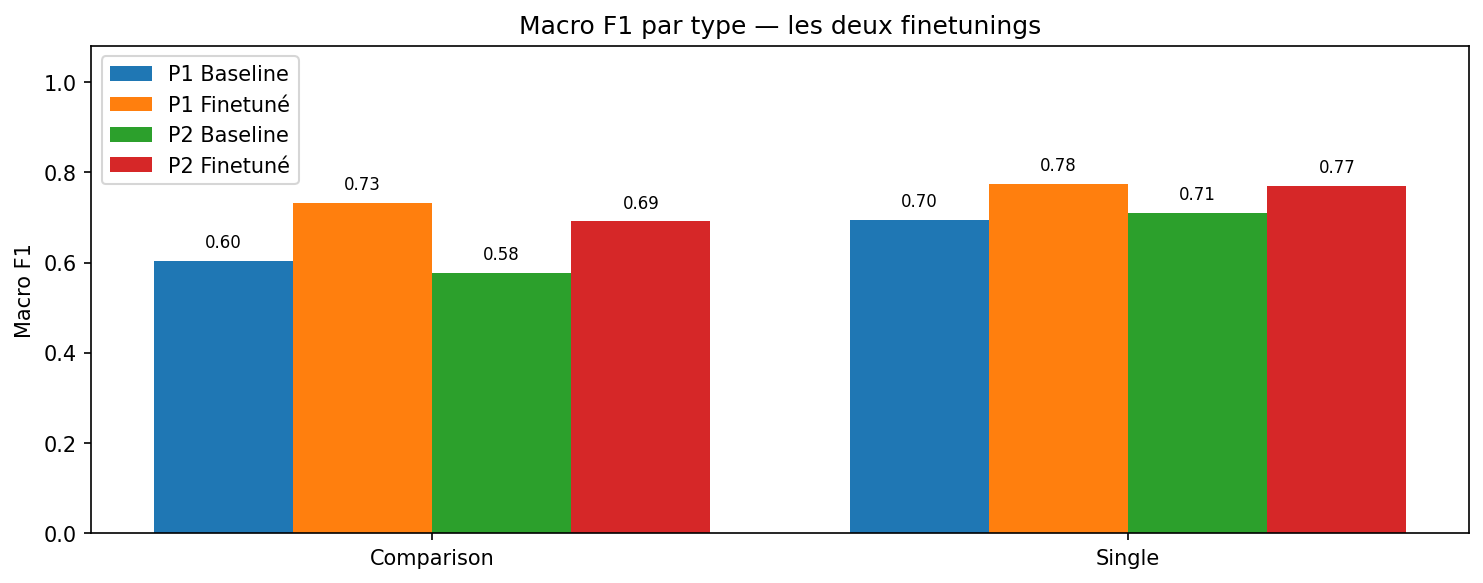
\includegraphics[width=0.9\linewidth]{02_accuracy_par_type.png}
\caption{Accuracy par type de tâche (Single / Comparison) pour les baselines et modèles fine-tunés (Prompt 1 et Prompt 2).}
\label{fig:nli4ct-accuracy-type}
\end{figure}

\begin{figure}[H]
\centering
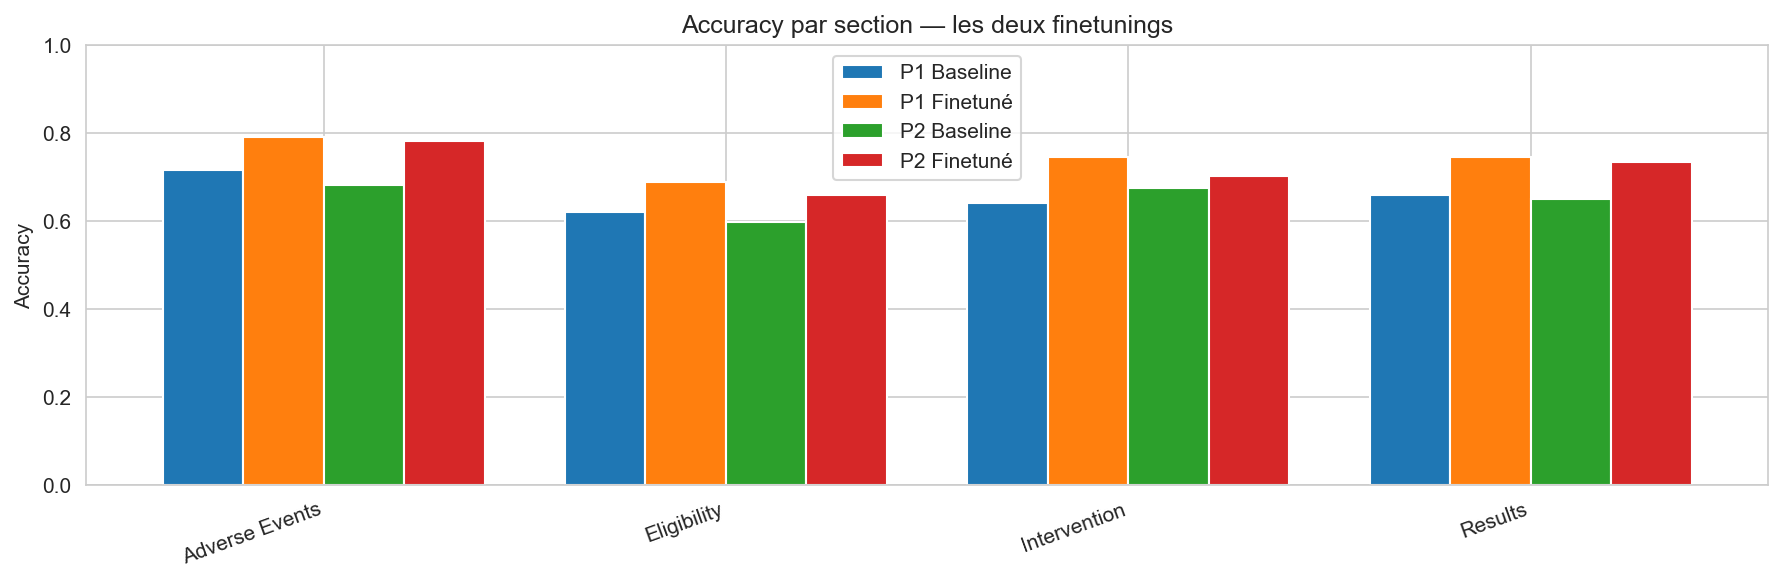
\includegraphics[width=0.9\linewidth]{03_accuracy_par_section.png}
\caption{Accuracy par section de protocole pour les baselines et modèles fine-tunés (Prompt 1 et Prompt 2).}
\label{fig:nli4ct-accuracy-section}
\end{figure}

Par ailleurs, le fine-tuning introduit des \textbf{régressions} (exemples corrects en baseline, erronés après affinage) et des \textbf{améliorations} (erronés en baseline, corrects après affinage)~: pour le Prompt 1 on observe 60 régressions et 102 améliorations~; pour le Prompt 2, 60 régressions et 93 améliorations. Le bilan net reste positif pour les deux prompts. Une explication probable des régressions est que les \textbf{baselines prédissent en majorité la classe Contradiction}~: lorsqu'une prédiction baseline correcte était «~contradiction~», l'affinage peut parfois faire basculer le modèle vers «~entailment~» et ainsi créer une régression. Les quatre matrices de confusion (P1 Baseline, P1 Fine-tuné, P2 Baseline, P2 Fine-tuné) reportées en figure~\ref{fig:nli4ct-confusion} illustrent ce déséquilibre des baselines vers la contradiction et le rééquilibrage apporté par le fine-tuning.

\begin{figure}[H]
\centering
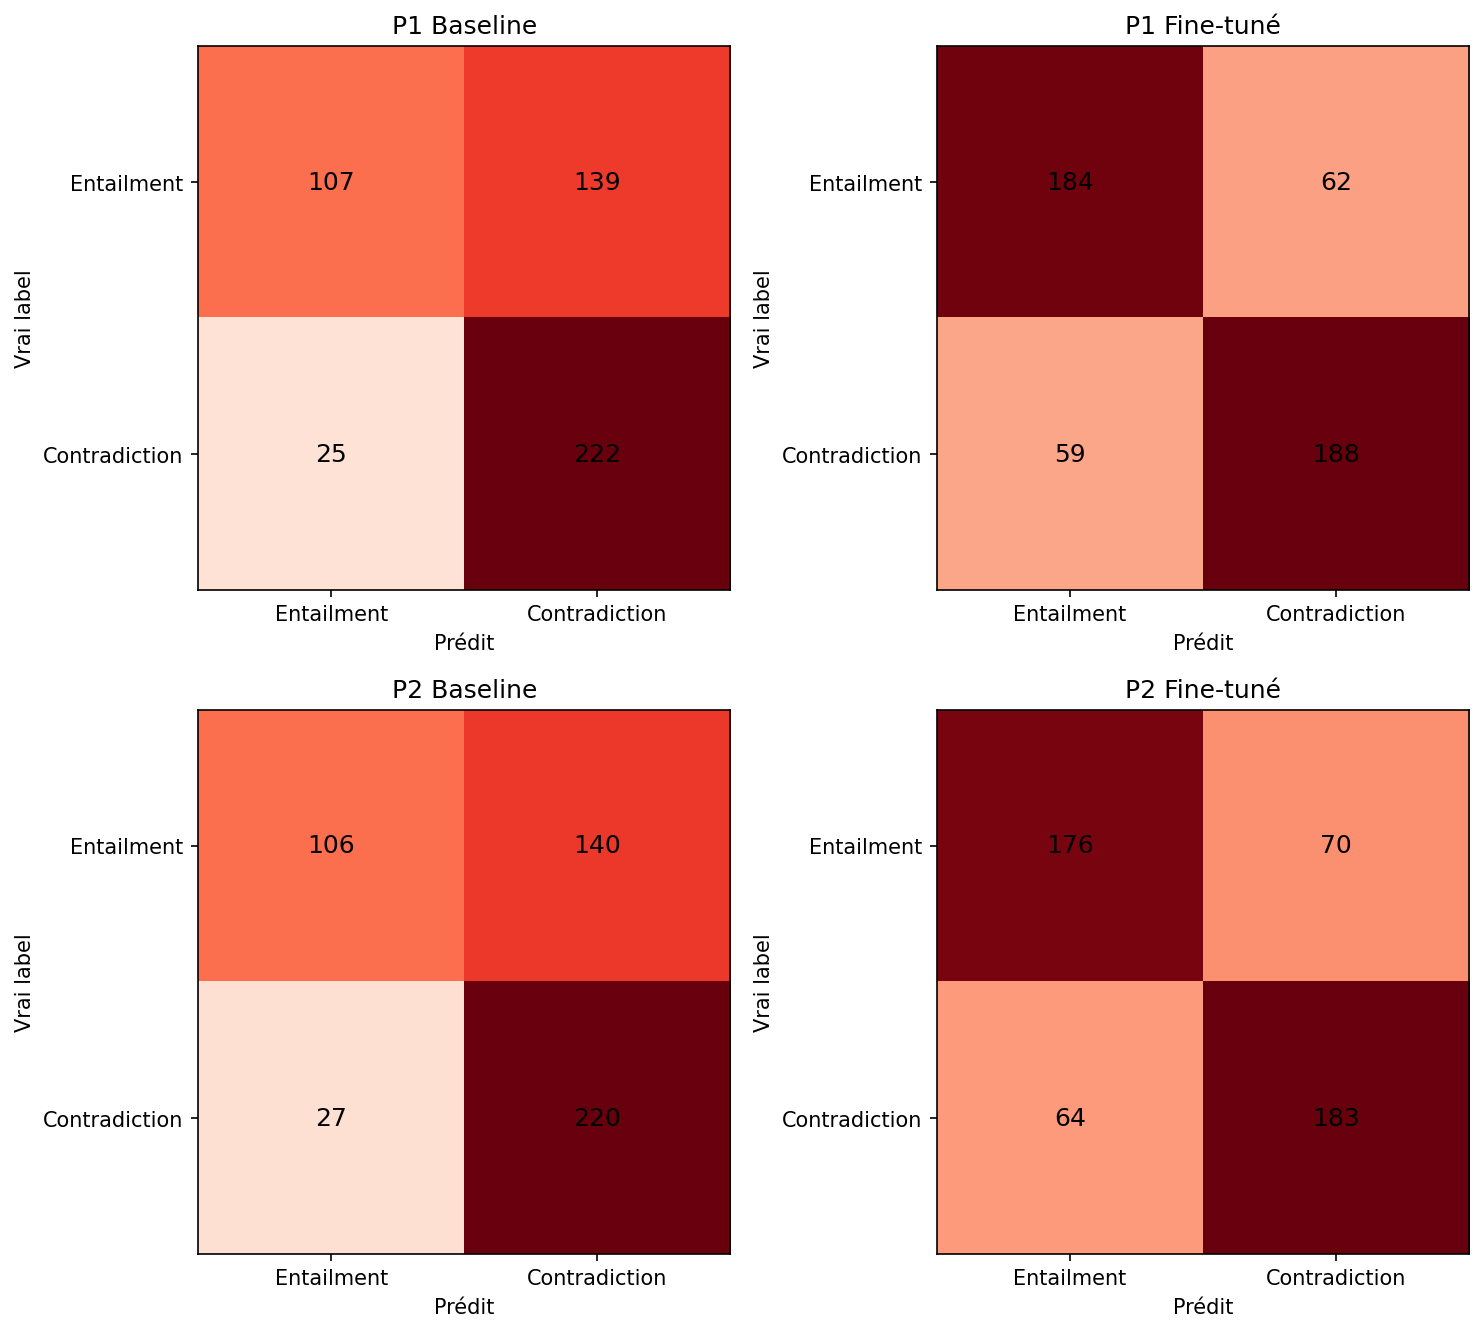
\includegraphics[width=0.7\linewidth]{fig_nli4ct_confusion.png}
\caption{Matrices de confusion pour P1 Baseline, P1 Fine-tuné, P2 Baseline et P2 Fine-tuné (calculées à partir des fichiers \texttt{resultats\_*}\, des dossiers Prompt\,1 et Prompt\,2). Les baselines tendent à prédire majoritairement Contradiction~; le fine-tuning rééquilibre les prédictions, ce qui peut expliquer une partie des régressions (exemples où la baseline correcte en contradiction devient erronée après affinage).}
\label{fig:nli4ct-confusion}
\end{figure}

L'analyse par \textbf{longueur de prompt} est donnée en figures~\ref{fig:nli4ct-longueur} et~\ref{fig:nli4ct-longueur-courbe}. Les données ont été découpées en sous-ensembles (\emph{bins}) de la façon suivante~: pour la figure~\ref{fig:nli4ct-longueur}, la longueur du prompt (en tokens) est partagée en \textbf{terciles} (quantiles à 1/3 et 2/3), ce qui définit trois bins «~Court~», «~Moyen~» et «~Long~»~; pour la figure~\ref{fig:nli4ct-longueur-courbe}, les exemples sont répartis en \textbf{15 bins} selon le rang centile de leur longueur (\emph{rank percentile}), puis l'accuracy est calculée dans chaque bin et reportée en fonction de la longueur moyenne du bin. Les performances restent stables ou s'améliorent avec la longueur pour les modèles affinés, sans dégradation systématique sur les prompts les plus longs.

\begin{figure}[H]
\centering
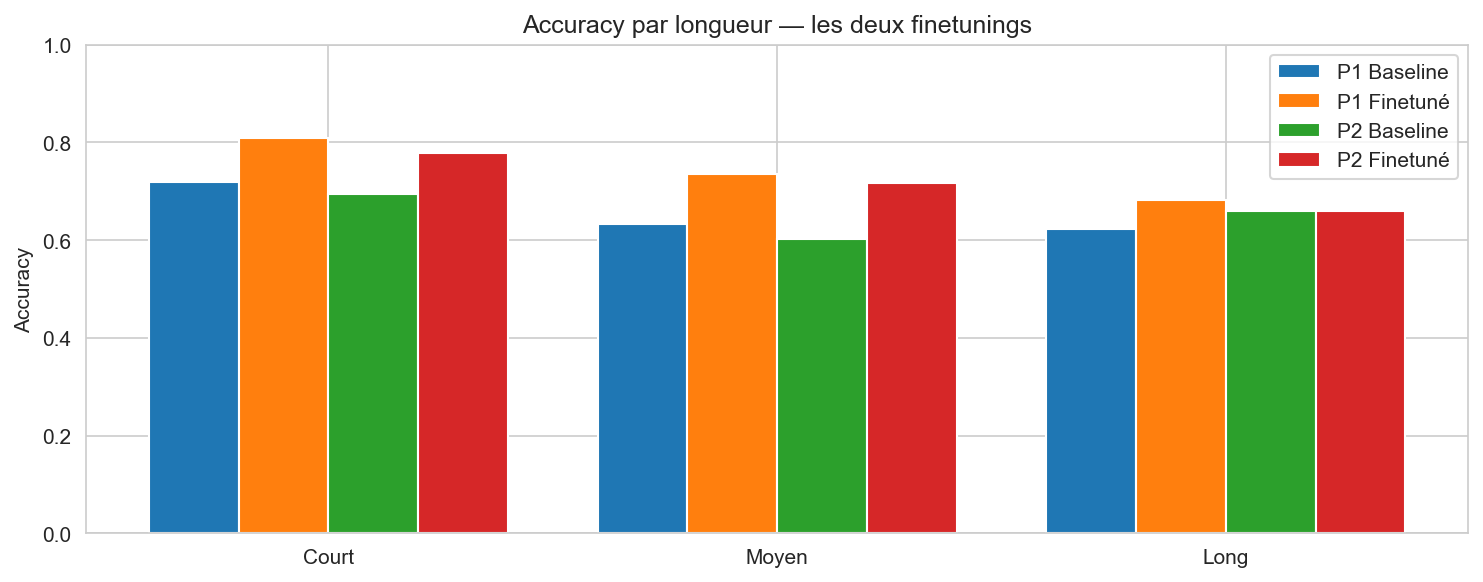
\includegraphics[width=0.9\linewidth]{04_accuracy_par_longueur.png}
\caption{Accuracy par bin de longueur (terciles~: Court / Moyen / Long) pour les baselines et modèles fine-tunés.}
\label{fig:nli4ct-longueur}
\end{figure}

\begin{figure}[H]
\centering
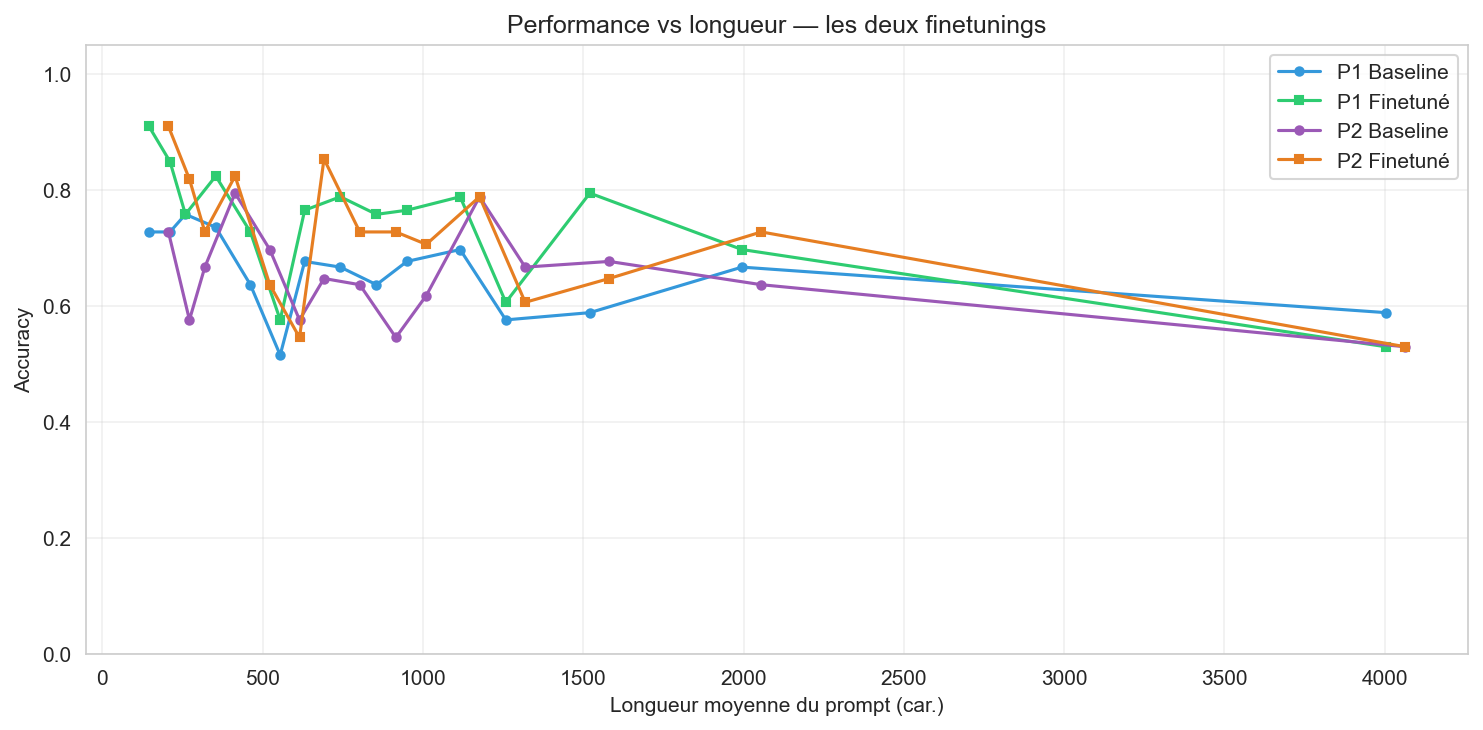
\includegraphics[width=0.9\linewidth]{04b_accuracy_vs_longueur_courbe.png}
\caption{Évolution de l'accuracy en fonction de la longueur du prompt (15 bins par rang centile, courbe lissée) pour les deux fine-tunings.}
\label{fig:nli4ct-longueur-courbe}
\end{figure}

\paragraph{Trois stratégies few-shot.}
Les trois stratégies few-shot (sélection par type et section, KATE, similarité cosine) atteignent des précisions du même ordre~: \textbf{72,0}\,\% pour la sélection par type et section, \textbf{71,4}\,\% pour KATE, \textbf{71,0}\,\% pour Cosine. Aucune ne dépasse le fine-tuning Prompt 1 (74,2\,\%), mais elles se situent au niveau du fine-tuning Prompt 2 ou légèrement en dessous, sans aucun ré-entraînement. La stratégie par type et section est légèrement en tête des trois. La figure~\ref{fig:nli4ct-fewshot-type-section} (partie 5b de l'analyse few-shot) présente la performance des trois stratégies par \textbf{type de tâche} et par \textbf{section de protocole} dans un même graphique~: les trois courbes ou barres sont très proches pour chaque sous-groupe, ce qui \textbf{justifie que les trois stratégies few-shot se comportent de manière très similaire} selon le type et la section, avec des variations limitées entre type+section, KATE et Cosine.

\begin{figure}[H]
\centering
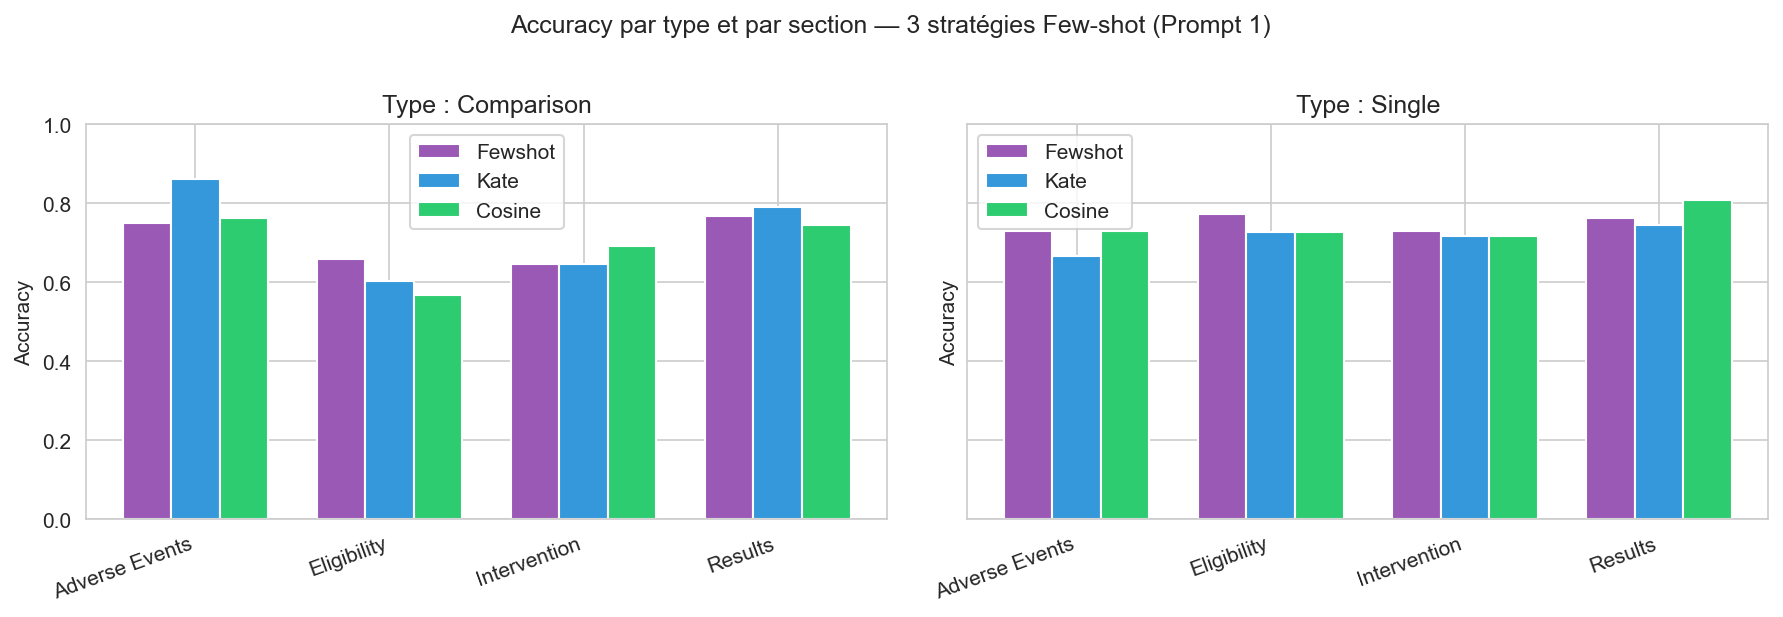
\includegraphics[width=0.9\linewidth]{02b_accuracy_type_et_section.png}
\caption{Performance des trois stratégies few-shot (type+section, KATE, cosine) par type de tâche et par section de protocole. Les trois stratégies montrent des profils très proches, justifiant un comportement similaire.}
\label{fig:nli4ct-fewshot-type-section}
\end{figure}

\paragraph{Synthèse comparative des cinq approches.}
Le fine-tuning Prompt 1 est le plus performant (74,2\,\%), suivi du fine-tuning Prompt 2 (71,8\,\%) et des trois stratégies few-shot (71,0--72,0\,\%). Les approches few-shot offrent un compromis intéressant~: précision proche du second fine-tuning, sans coût d'affinage. Pour la suite de l'analyse (section suivante), on se concentre sur la stratégie \textbf{KATE}~: les trois stratégies few-shot étant de performance très similaire, le choix de KATE se justifie par le fait que c'est une \textbf{méthode générale}, réutilisable sur d'autres tâches (y compris NLI4PR), et dont le principe — sélection d'exemples par similarité sémantique — a une interprétation claire. La section suivante (analyse d'erreurs) détaille où les modèles se trompent, où ils sont d'accord, et dans quelle mesure le fine-tuning Prompt 1 et KATE se complètent.

\subsection{Résultats NLI4PR}
L'évaluation NLI4PR porte sur 3156 exemples de test (1578 en langage patient POL et 1578 en langage médical), avec quatre familles de configurations~: les trois prompts (\textbf{NLI}, \textbf{Clinical Matching}, \textbf{CoT}) en \textbf{baseline} (sans affinage) et en \textbf{finetuné}, ainsi que la stratégie \textbf{few-shot KATE} (sans entraînement). Le tableau~\ref{tab:nli4pr-accuracy} synthétise l'accuracy (\,\%) en Global, POL et MEDICAL pour toutes ces configurations.

\begin{table}[htbp]
\centering
\caption{Précision (accuracy, \,\%) sur NLI4PR — Global (3156 ex.), POL (1578 ex.) et MEDICAL (1578 ex.).}
\label{tab:nli4pr-accuracy}
\begin{tabular}{lccc}
\toprule
Configuration & Global & POL & MEDICAL \\
\midrule
NLI Baseline & 55,7 & 53,8 & 57,6 \\
NLI Finetuné & \textbf{68,9} & 68,3 & 69,6 \\
Clinical Matching Baseline & 66,2 & 65,0 & 67,4 \\
Clinical Matching Finetuné & 72,8 & 73,3 & 72,4 \\
CoT Baseline & 72,2 & 70,5 & 74,0 \\
CoT Finetuné & \textbf{73,8} & 73,4 & \textbf{74,2} \\
Few-shot KATE & 66,2 & 65,6 & 66,7 \\
\bottomrule
\end{tabular}
\end{table}

\paragraph{Synthèse des performances.}
Le \textbf{finetuning améliore nettement} les trois prompts par rapport à leurs baselines. Le gain est le plus marqué pour le prompt \textbf{NLI}~: +13,2 points en global (55,7\,\% $\rightarrow$ 68,9\,\%), avec des améliorations similaires en POL et MEDICAL. Les prompts Clinical Matching et CoT partent de baselines déjà plus élevées (66,2\,\% et 72,2\,\%) et gagnent encore respectivement +6,6 et +1,6 points en global après affinage. Au final, le \textbf{CoT finetuné} obtient la meilleure accuracy globale (73,8\,\%) et en MEDICAL (74,2\,\%)~; le Clinical Matching finetuné reste très proche (72,8\,\% global, 73,3\,\% en POL). La stratégie \textbf{few-shot KATE} a également été évaluée sur NLI4PR (66,2\,\% en global, 65,6\,\% en POL, 66,7\,\% en MEDICAL). Les résultats restent nettement inférieurs à toutes les configurations par prompt (finetuné) sur ce jeu de données~; nous ne nous sommes donc pas concentrés sur cette approche pour NLI4PR.

\paragraph{Comparaison par type de langage (POL vs MEDICAL).}
En baseline, les trois prompts performent légèrement mieux sur le sous-ensemble \textbf{MEDICAL} que sur \textbf{POL}, avec des écarts de l'ordre de 2 à 4 points. Après finetuning, les écarts entre POL et MEDICAL se réduisent~: le CoT finetuné atteint 73,4\,\% en POL et 74,2\,\% en MEDICAL. Les figures~\ref{fig:nli4pr-compare-baseline} et~\ref{fig:nli4pr-compare-finetune} illustrent la comparaison des trois prompts en baseline et en finetuné (Global, POL, MEDICAL).

\begin{figure}[H]
\centering
\IfFileExists{figures_nli4pr/compare_all_baseline_accuracy.png}{%
  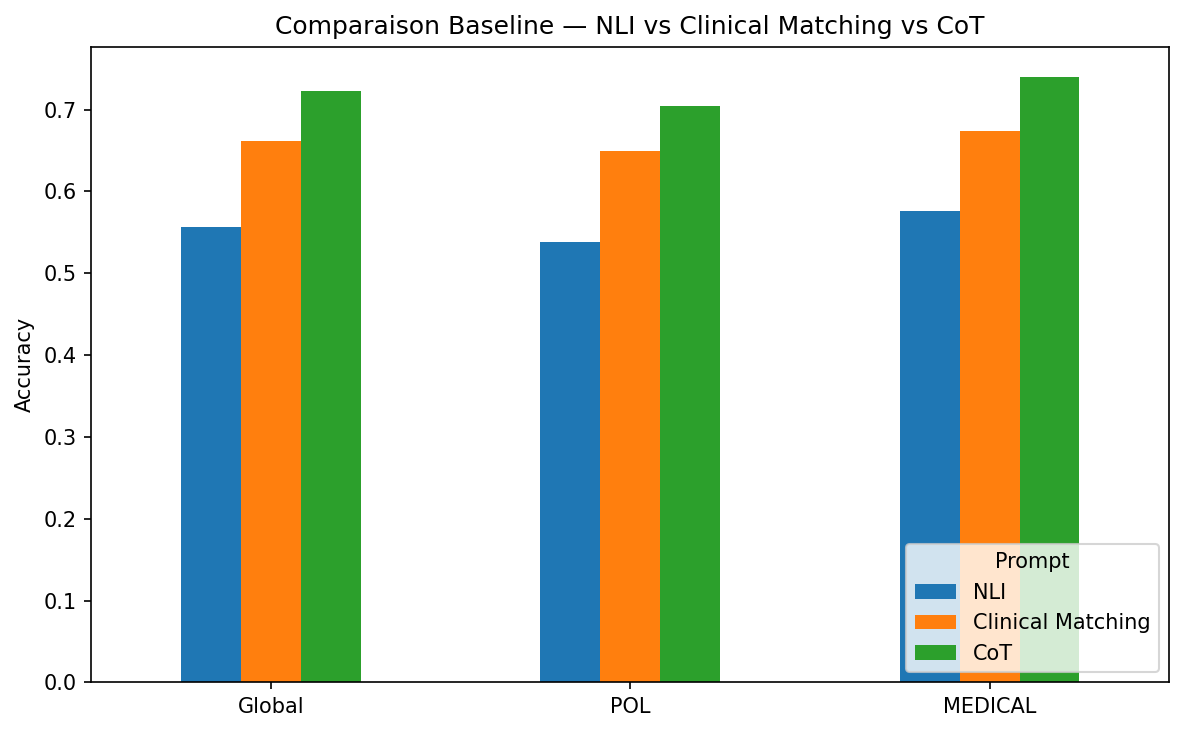
\includegraphics[width=0.72\linewidth]{figures_nli4pr/compare_all_baseline_accuracy.png}%
}{\fbox{\parbox{0.72\linewidth}{\centering\small [Exécuter les notebooks NLI4PR puis \texttt{copy\_figures\_nli4pr.bat} pour générer la figure.]}}}
\caption{Accuracy des trois prompts (NLI, Clinical Matching, CoT) en \textbf{baseline} — Global, POL et MEDICAL.}
\label{fig:nli4pr-compare-baseline}
\end{figure}

\begin{figure}[H]
\centering
\IfFileExists{figures_nli4pr/compare_all_finetuning_accuracy.png}{%
  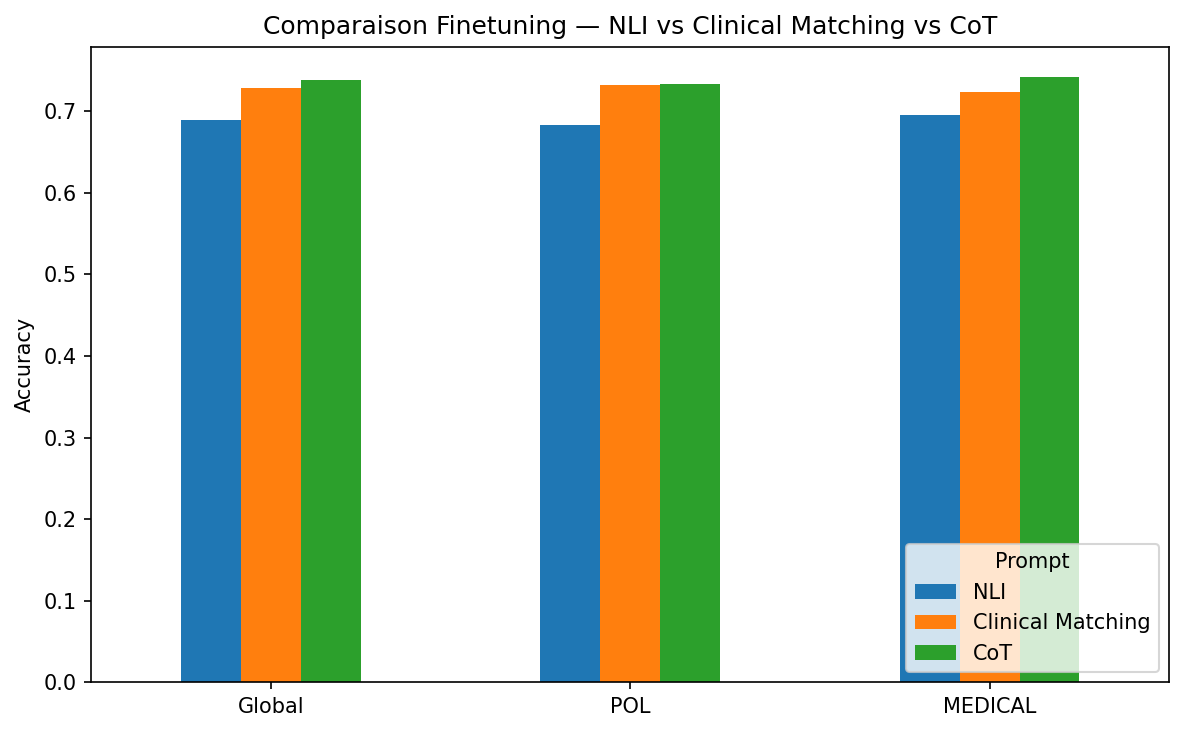
\includegraphics[width=0.72\linewidth]{figures_nli4pr/compare_all_finetuning_accuracy.png}%
}{\fbox{\parbox{0.72\linewidth}{\centering\small [Figure~: \texttt{compare\_all\_finetuning\_accuracy.png}]}}}
\caption{Accuracy des trois prompts (NLI, Clinical Matching, CoT) \textbf{finetunés} — Global, POL et MEDICAL. Le CoT finetuné obtient les meilleurs scores.}
\label{fig:nli4pr-compare-finetune}
\end{figure}

\paragraph{Baseline vs Finetuné par prompt.}
Pour chaque prompt, le finetuning apporte plus d'améliorations que de régressions. Par exemple, pour le NLI~: 1108 exemples passent de faux (baseline) à corrects (finetuné) contre 691 régressions (correct en baseline, faux après affinage), soit un bilan net de +417 exemples corrects. Les figures~\ref{fig:nli4pr-nli-bf},~\ref{fig:nli4pr-cm-bf} et~\ref{fig:nli4pr-cot-bf} montrent les courbes baseline vs finetuné pour les trois prompts (accuracy Global, POL, MEDICAL). Une matrice de confusion typique (CoT finetuné, combined) est donnée en figure~\ref{fig:nli4pr-cot-confusion} pour illustrer la répartition des prédictions Entailment / Contradiction.

\begin{figure}[H]
\centering
\IfFileExists{figures_nli4pr/nli_compare_baseline_finetune_accuracy.png}{%
  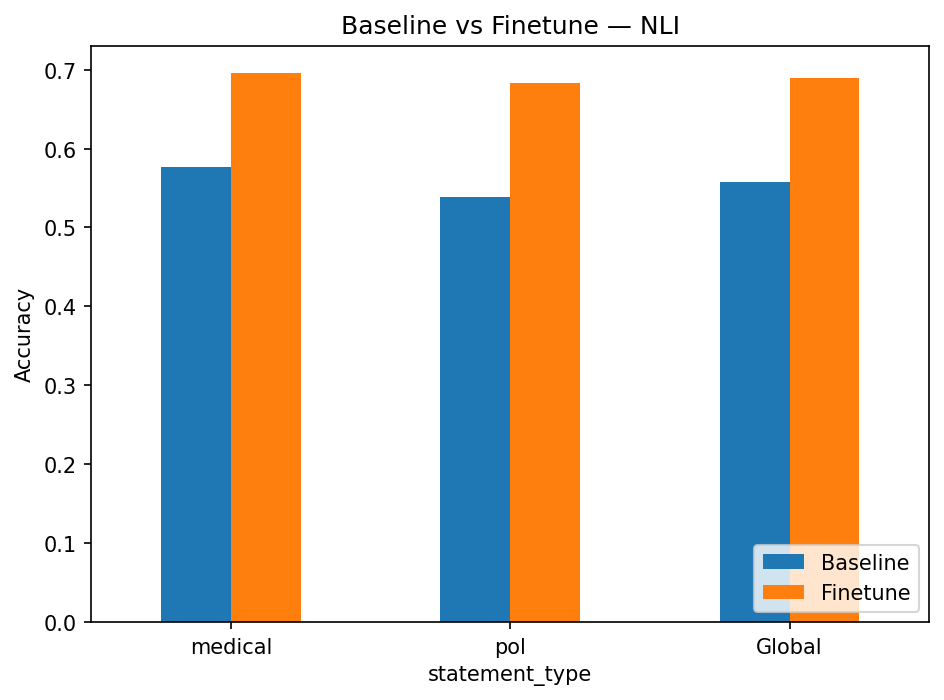
\includegraphics[width=0.68\linewidth]{figures_nli4pr/nli_compare_baseline_finetune_accuracy.png}%
}{\fbox{\parbox{0.68\linewidth}{\centering\small [\texttt{nli\_compare\_baseline\_finetune\_accuracy.png}]}}}
\caption{Baseline vs Finetuné — prompt \textbf{NLI}. Gain important du finetuning en Global, POL et MEDICAL.}
\label{fig:nli4pr-nli-bf}
\end{figure}

\begin{figure}[H]
\centering
\IfFileExists{figures_nli4pr/clinical_matching_compare_baseline_finetune_accuracy.png}{%
  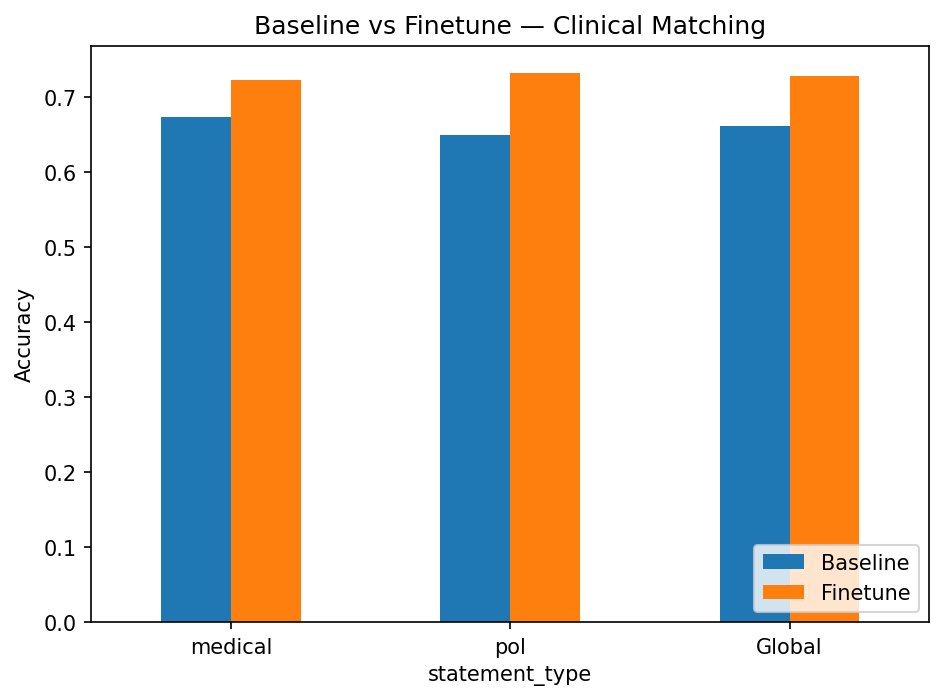
\includegraphics[width=0.68\linewidth]{figures_nli4pr/clinical_matching_compare_baseline_finetune_accuracy.png}%
}{\fbox{\parbox{0.68\linewidth}{\centering\small [\texttt{clinical\_matching\_compare\_baseline\_finetune\_accuracy.png}]}}}
\caption{Baseline vs Finetuné — prompt \textbf{Clinical Matching}.}
\label{fig:nli4pr-cm-bf}
\end{figure}

\begin{figure}[H]
\centering
\IfFileExists{figures_nli4pr/cot_compare_baseline_finetune_accuracy.png}{%
  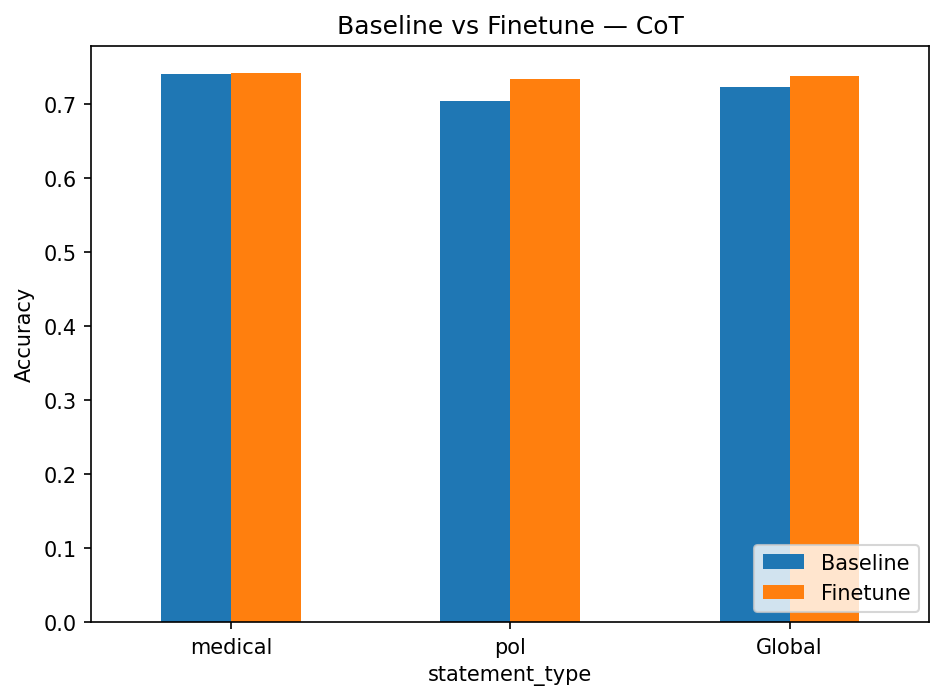
\includegraphics[width=0.68\linewidth]{figures_nli4pr/cot_compare_baseline_finetune_accuracy.png}%
}{\fbox{\parbox{0.68\linewidth}{\centering\small [\texttt{cot\_compare\_baseline\_finetune\_accuracy.png}]}}}
\caption{Baseline vs Finetuné — prompt \textbf{CoT}. La baseline CoT est déjà élevée~; le finetuning apporte un gain modéré mais consistant.}
\label{fig:nli4pr-cot-bf}
\end{figure}

\begin{figure}[H]
\centering
\IfFileExists{figures_nli4pr/cot_finetune_confusion_combined.png}{%
  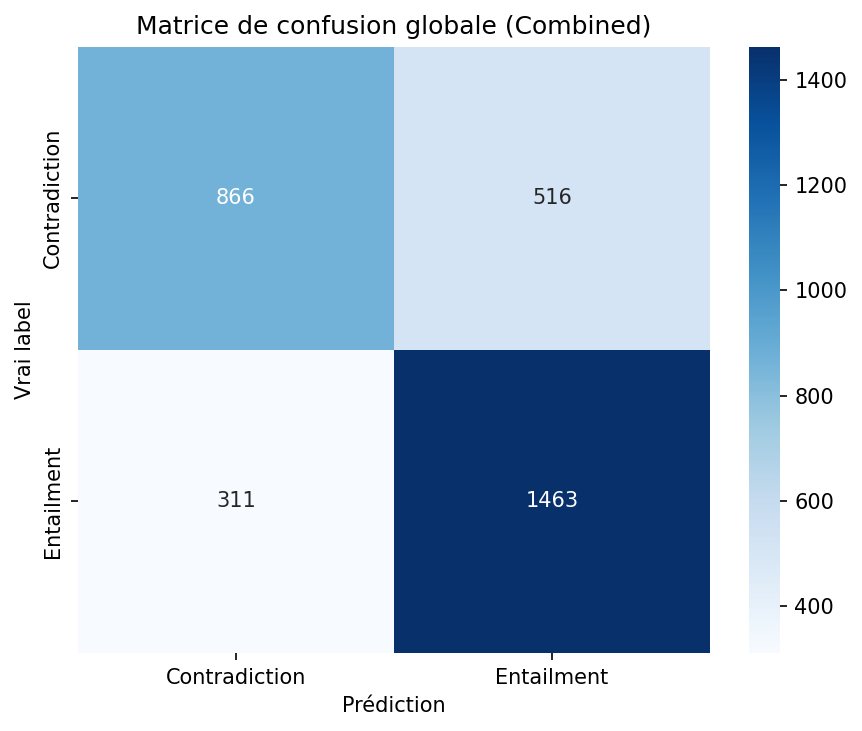
\includegraphics[width=0.58\linewidth]{figures_nli4pr/cot_finetune_confusion_combined.png}%
}{\fbox{\parbox{0.58\linewidth}{\centering\small [\texttt{cot\_finetune\_confusion\_combined.png}]}}}
\caption{Matrice de confusion — CoT finetuné, ensemble combined (POL + MEDICAL).}
\label{fig:nli4pr-cot-confusion}
\end{figure}

\paragraph{Noyau dur d'erreurs.}
Lorsque \emph{les trois} modèles \textbf{baseline} se trompent ensemble (237 exemples en POL, 174 en MEDICAL), ils prédisent à tort \textbf{Contradiction} dans la grande majorité des cas~: le vrai label est Entailment dans environ \textbf{92\,\%} des cas en POL et \textbf{88\,\%} en MEDICAL. Les baselines ont donc une tendance à sous-déclarer l'éligibilité. À l'inverse, lorsque les trois modèles \textbf{finetunés} se trompent ensemble (196 en POL, 174 en MEDICAL), le vrai label est majoritairement \textbf{Contradiction} (environ 75\,\% en POL et 80\,\% en MEDICAL)~: les modèles finetunés tendent alors à prédire à tort Entailment. Nous choisissons \textbf{123 candidats} pour l'analyse d'erreurs NLI4PR (section suivante) provenant de l'intersection de ces indices en POL et en MEDICAL pour les modèles \textbf{finetunés} (même patient en erreur dans les deux formulations). Nous ciblons les erreurs du finetuning car c'est là que les meilleurs résultats sont obtenus~; l'analyse d'erreurs NLI4PR (section suivante) porte sur ce noyau dur.

\section{Analyse d'erreurs}

\subsection{Analyse d'erreurs NLI4CT}
L'analyse d'erreurs porte sur trois axes~: la convergence des erreurs entre les deux fine-tunings (Prompt 1 et Prompt 2), entre les trois stratégies few-shot, puis la complémentarité entre le meilleur fine-tuning (Prompt 1) et le meilleur few-shot (KATE). Les effectifs et répartitions ci-dessous proviennent des comparaisons systématiques réalisées sur le Gold test (500 exemples).

\paragraph{Convergence des erreurs entre les deux fine-tunings.}
On compare les prédictions du \textbf{Prompt 1 fine-tuné} et du \textbf{Prompt 2 fine-tuné} sur les 500 exemples. La répartition des quatre cas d'accord/désaccord est la suivante~: \textbf{333 exemples où les deux ont raison}, \textbf{103 où les deux se trompent}, \textbf{38 où seul le Prompt 1 a raison} (P2 en erreur) et \textbf{26 où seul le Prompt 2 a raison} (P1 en erreur). Les deux modèles sont donc d'accord sur une large majorité des cas (333 + 103 = 436, soit 87,2\,\%). Les désaccords (64 exemples au total) sont légèrement en faveur du Prompt 1 (38 contre 26), cohérent avec sa meilleure accuracy globale. Les \textbf{103 cas où les deux se trompent} constituent un noyau dur commun aux deux formulations de prompt~; leur répartition par \textbf{section de protocole} montre une surreprésentation dans certaines sections (par ex. Eligibility, Intervention, Adverse Events, Results), ce qui indique des zones où l'affinage reste insuffisant pour les deux configurations. La répartition par \textbf{type de tâche} (Single vs Comparison) dans ces 103 cas permet d'identifier si les erreurs communes concernent davantage les inférences sur un seul critère ou les comparaisons entre critères. Par ailleurs, comme indiqué en résultats, le fine-tuning introduit 60 régressions et 102 améliorations pour le Prompt 1, 60 régressions et 93 améliorations pour le Prompt 2~: les améliorations l'emportent nettement, mais les régressions ciblent des exemples que les baselines géraient correctement et méritent une analyse qualitative (par ex. confusion Entailment / Contradiction). La figure~\ref{fig:nli4ct-twoft-section} synthétise la répartition des cas «~les deux finetunings se trompent~» et «~les deux finetunings ont raison~» par section de protocole.

\begin{figure}[H]
\centering
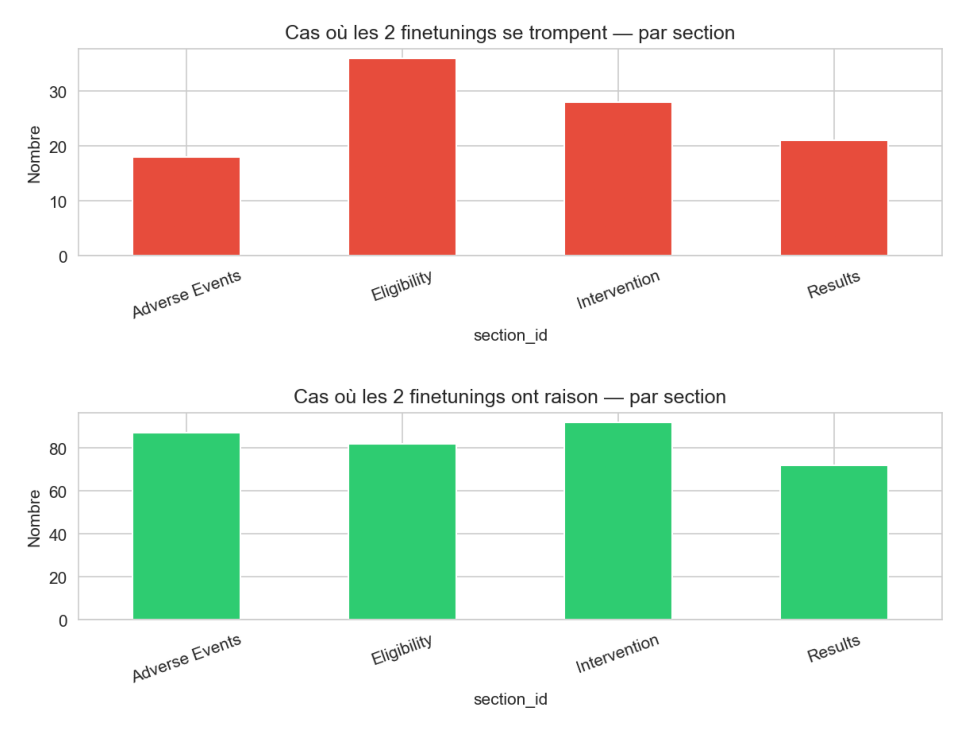
\includegraphics[width=0.9\linewidth]{fig_twoft_by_section.png}
\caption{Répartition par section de protocole des cas où les deux modèles fine-tunés (Prompt 1 et Prompt 2) se trompent (en haut) et des cas où les deux ont raison (en bas). Les deux modèles sont nettement plus susceptibles de se tromper sur les sections \textit{Eligibility} et \textit{Intervention} que sur \textit{Results} ou \textit{Adverse Events}.}
\label{fig:nli4ct-twoft-section}
\end{figure}

On observe que, parmi les 103 cas où les deux modèles se trompent, les sections \textit{Eligibility} et \textit{Intervention} concentrent une part plus importante des erreurs communes que les sections \textit{Results} et \textit{Adverse Events}, alors que ces dernières regroupent davantage de cas correctement traités. Autrement dit, même après affinage, les deux modèles restent \textbf{plus fragiles sur les tâches d'éligibilité et d'intervention} que sur les tâches liées aux résultats ou aux événements indésirables, ce qui renforce l'intérêt d'analyses spécifiques sur ces sections et d'une étude complémentaire focalisée sur l'éligibilité (NLI4PR).

\paragraph{Convergence des erreurs entre les trois stratégies few-shot.}
Une analyse similaire porte sur les \textbf{trois stratégies few-shot} (sélection par type et section, KATE, similarité cosine). En termes d'accord global~: \textbf{264 exemples où les trois ont raison}, \textbf{117 où les trois se trompent}, et \textbf{119 en désaccord} (une ou deux stratégies correctes, les autres en erreur). Les effectifs d'erreurs par stratégie sont~: 140 pour la sélection par type et section, 143 pour KATE, 145 pour Cosine. Les chevauchements d'erreurs deux à deux sont importants~: 97 erreurs communes entre la stratégie par type/section et KATE, 100 entre type/section et Cosine, 112 entre KATE et Cosine. KATE et Cosine, toutes deux basées sur la similarité sémantique, partagent donc le plus d'erreurs (112), ce qui suggère qu'ils échouent sur des profils d'exemples proches. La stratégie par type et section partage un peu moins d'erreurs avec chacune d'elles (97 et 100), tout en ayant légèrement moins d'erreurs au total (140). Les 117 cas où \emph{les trois} se trompent forment un sous-ensemble difficile pour l'ensemble des configurations few-shot~; leur répartition par type de tâche et par section de protocole (comme dans les notebooks) permet d'identifier les zones où les trois stratégies sont limitées. En synthèse, les trois approches few-shot convergent sur une grande partie des réponses correctes et des erreurs, avec des désaccords (119) qui restent limités~; la stratégie par type et section reste la plus précise (72\,\%) avec un nombre d'erreurs légèrement inférieur.

\paragraph{Complémentarité fine-tuning Prompt 1 et few-shot KATE.}
On restreint l'analyse aux prédictions du \textbf{fine-tuning Prompt 1} (74,2\,\%) et du \textbf{few-shot KATE} (71,4\,\%), les deux approches les plus performantes dans chaque famille. Sur le Gold test~: \textbf{299 exemples où les deux ont raison}, \textbf{71 où les deux se trompent}, \textbf{72 où seul le fine-tuning a raison} et \textbf{58 où seul KATE a raison}. L'accord domine (299 + 71 = 370, 74\,\%), mais la complémentarité est nette~: 130 exemples (72 + 58) où un seul des deux a raison, chaque approche compensant partiellement l'autre. Pour interpréter ces écarts, une \textbf{analyse linguistique} a été menée sur les quatre sous-ensembles, avec les indicateurs suivants~: chevauchement lexical (Jaccard, coverage), densité numérique (chiffres, pourcentages, unités), présence de négations, longueur de la prémisse. Le tableau~\ref{tab:nli4ct-moyennes-4cas} résume les moyennes de ces indicateurs pour chacun des quatre cas.

\begin{table}[htbp]
\centering
\caption{Moyennes des indicateurs linguistiques par cas (fine-tuning Prompt 1 vs few-shot KATE).}
\label{tab:nli4ct-moyennes-4cas}
\scriptsize
\resizebox{\linewidth}{!}{%
\begin{tabular}{lrrrrrr}
\toprule
Cas & Jaccard lex. & Couverture & Densité num. & Négations & Mots prémisse & Mots hypothèse \\
\midrule
Les 2 corrects & 0,1045 & 0,3354 & 41,08 & 0,82 & 113,43 & 21,50 \\
Les 2 en erreur & 0,1050 & 0,3799 & 39,59 & 2,31 & 169,06 & 21,51 \\
P1\textsuperscript{$\checkmark$} KATE\textsuperscript{$\times$} & 0,1073 & 0,3553 & 42,89 & 1,03 & 124,26 & 22,54 \\
P1\textsuperscript{$\times$} KATE\textsuperscript{$\checkmark$} & 0,1004 & 0,3958 & 61,24 & 1,81 & 220,84 & 24,47 \\
\bottomrule
\end{tabular}%
}
\end{table}

Les tests de \textbf{Kruskal-Wallis} indiquent que les quatre groupes se distinguent significativement par la \textbf{densité numérique} (\texttt{numeric\_total}) et la \textbf{longueur de la prémisse} (\texttt{words\_premise}). Les cas où \textbf{les deux se trompent} (71) contiennent en moyenne \textbf{plus de négations} que les cas où les deux ont raison (test de Mann-Whitney, $p < 0{,}05$)~: les deux approches échouent plus souvent sur des contradictions à base de négations explicites. À l'inverse, dans le sous-ensemble \textbf{P1 en erreur et KATE correct} (58 exemples), les exemples ont une \textbf{densité numérique plus élevée} et des \textbf{prémisses plus longues} ($p < 0{,}05$)~: le few-shot KATE, avec des exemples sémantiquement proches, semble mieux exploiter le contexte numérique et les critères longs. Dans le sous-ensemble \textbf{P1 correct et KATE en erreur} (72 exemples), le profil (moins numérique, prémisses plus courtes en moyenne) correspond au domaine où le fine-tuning tire mieux parti de l'affinage. En pratique, ces résultats suggèrent qu'un \textbf{système hybride} ou un \textbf{choix ciblé} (par ex. préférer KATE sur les cas très numériques ou à longue prémisse, le fine-tuning Prompt 1 ailleurs) pourrait tirer parti de cette complémentarité et potentiellement dépasser la précision de chaque approche seule.

\subsection{Analyse d'erreurs NLI4PR}

Une \textbf{analyse linguistique} a été menée sur notre selection de 123 candidats, en les comparant au reste des indices du jeu de test (comme pour NLI4CT). Les métriques utilisées sont~: chevauchement lexical (Jaccard), couverture lexicale, densité numérique (chiffres, pourcentages, unités), nombre de négations, longueur de la prémisse et du statement, et présence de mots-clés d'essai. Les tableaux~\ref{tab:nli4pr-linguistic-pol} et~\ref{tab:nli4pr-linguistic-med} résument les moyennes candidats vs autres (POL et MEDICAL). Les candidats se distinguent par des \textbf{prémisses plus courtes} (environ 198 mots vs 252 pour les autres), une \textbf{densité numérique plus faible} (environ 31--33 vs 37--40), et une \textbf{couverture lexicale légèrement plus basse}. En MEDICAL, les candidats ont en moyenne \textbf{plus de négations dans le statement} (1,72 vs 1,42). Ces profils suggèrent que le noyau dur d'erreurs correspond à des cas où les critères sont moins longs et moins chargés en données numériques, avec des formulations potentiellement plus ambiguës (négations). Les figures~\ref{fig:nli4pr-comparison-pol} et~\ref{fig:nli4pr-comparison-medical} illustrent la comparaison détaillée des métriques entre candidats et autres indices.

\begin{table}[H]
\centering
\caption{Moyennes des indicateurs linguistiques — candidats vs autres (POL).}
\label{tab:nli4pr-linguistic-pol}
\scriptsize
\begin{tabular}{lrrr}
\toprule
Indicateur & Candidats & Autres & $\Delta$ \\
\midrule
Longueur prémisse (mots) & 198 & 252 & $-53$ \\
Densité numérique totale & 30,9 & 37,3 & $-6{,}4$ \\
Couverture lexicale & 0,183 & 0,196 & $-0{,}012$ \\
Négations (statement) & 1,02 & 0,91 & $+0{,}10$ \\
\bottomrule
\end{tabular}
\end{table}

\begin{table}[H]
\centering
\caption{Moyennes des indicateurs linguistiques — candidats vs autres (MEDICAL).}
\label{tab:nli4pr-linguistic-med}
\scriptsize
\begin{tabular}{lrrr}
\toprule
Indicateur & Candidats & Autres & $\Delta$ \\
\midrule
Longueur prémisse (mots) & 198 & 252 & $-54$ \\
Densité numérique totale & 32,8 & 40,1 & $-7{,}3$ \\
Couverture lexicale & 0,213 & 0,233 & $-0{,}020$ \\
Négations (statement) & 1,72 & 1,42 & $+0{,}30$ \\
\bottomrule
\end{tabular}
\end{table}

\begin{figure}[H]
\centering
\IfFileExists{figures_nli4pr/comparison_detailed_pol.png}{%
  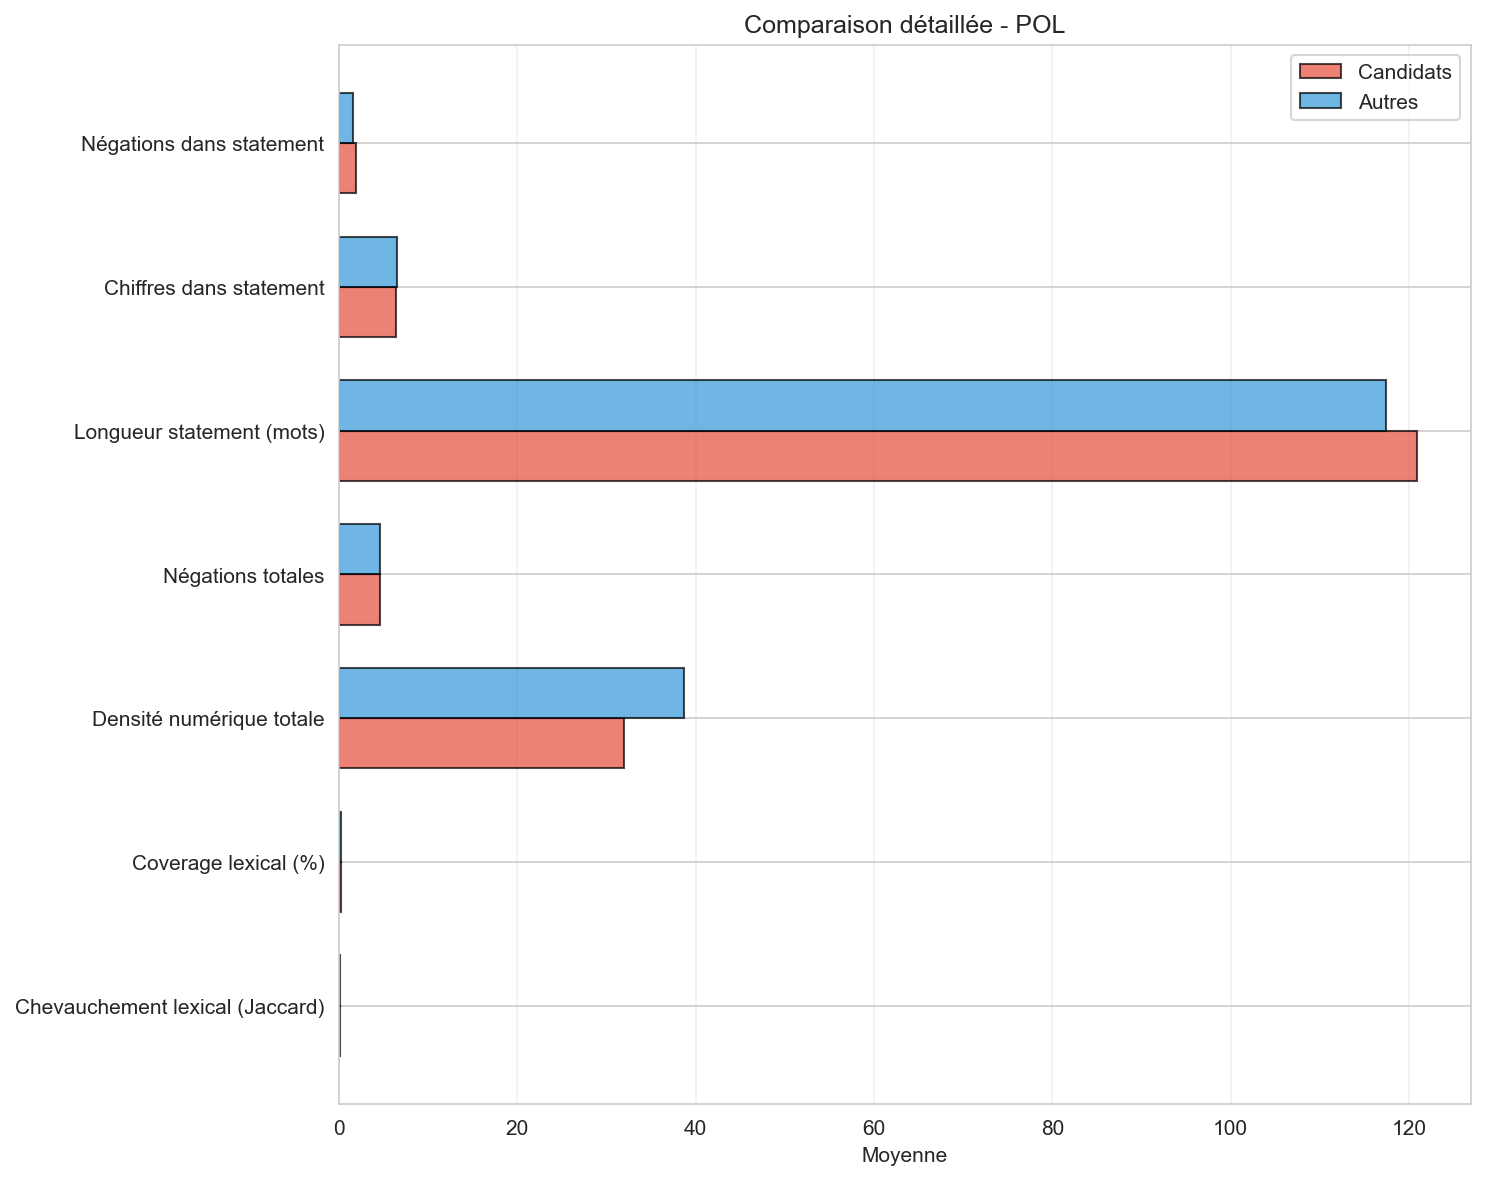
\includegraphics[width=0.72\linewidth]{figures_nli4pr/comparison_detailed_pol.png}%
}{\fbox{\parbox{0.72\linewidth}{\centering\small [\texttt{comparison\_detailed\_pol.png}]}}}
\caption{Comparaison des métriques linguistiques — candidats vs autres indices (POL).}
\label{fig:nli4pr-comparison-pol}
\end{figure}

\begin{figure}[H]
\centering
\IfFileExists{figures_nli4pr/comparison_detailed_medical.png}{%
  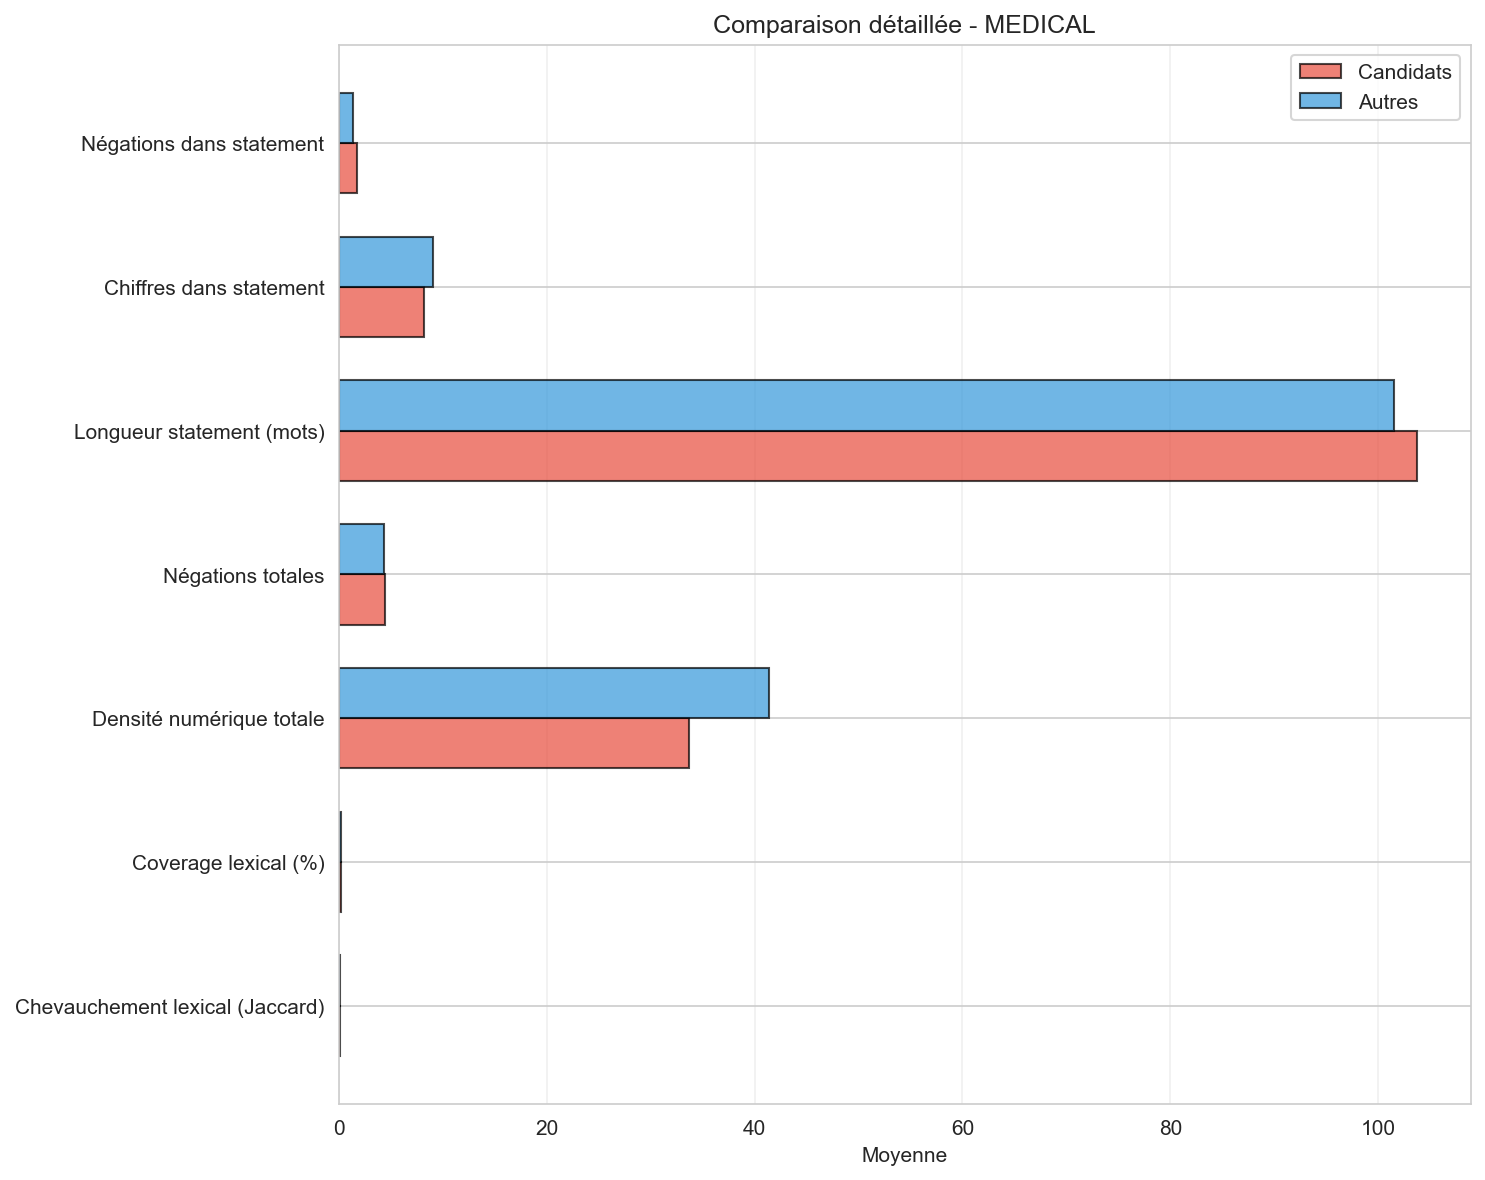
\includegraphics[width=0.72\linewidth]{figures_nli4pr/comparison_detailed_medical.png}%
}{\fbox{\parbox{0.72\linewidth}{\centering\small [\texttt{comparison\_detailed\_medical.png}]}}}
\caption{Comparaison des métriques linguistiques — candidats vs autres indices (MEDICAL).}
\label{fig:nli4pr-comparison-medical}
\end{figure}

En résumé, le finetuning réduit le nombre de cas «~tous faux~» (237 $\rightarrow$ 196 en POL) et rééquilibre les prédictions~; le résidu d'erreurs communes (123 candidats) correspond à un profil linguistique distinct (prémisses plus courtes, moins de densité numérique, davantage de négations en MEDICAL), ce qui peut orienter des améliorations ciblées (ex.~données d'entraînement complémentaires ou prompts adaptés à ces cas).

\section{Conclusion et perspectives}

\section{Limitations}

%%================================================================
\subsection{Rappels importants}
  \begin{itemize}
  \item Le style bibliographique tient compte des champs \verb!doi! et \verb!hal_id!. Des exemples sont donnés dans la bibliographie~\cite{pereira-warren:1983,Bernhard07,tellier:2008}. Voir également le fichier \verb!biblio.bib! fourni.
  \item Le \emph{package} \verb!hyperref! est chargé automatiquement par le fichier de style \verb!jeptaln2020.sty!. Certains \emph{packages} particuliers doivent être donc chargés avant, certains après, suivant les compatibilités avec \verb!hyperref! (voir les \href{http://distrib-coffee.ipsl.jussieu.fr/pub/mirrors/ctan/macros/latex/contrib/hyperref/doc/manual.html#x1-520009}{compatibilités dans la documentation}).
    \item Si vous utilisez les symboles utf-8 pour les guillements français, ne
pas oublier les espaces insécables \verb!~! après les guillemets
ouvrants ou avant les guillements fermants : « test »
(\verb!«~test~»!). Sinon, vous pouvez utiliser les commandes
\verb!\og!  et \verb!\fg! : \og test \fg{} (\verb!\og test \fg{}!).
\item Exemple d'utilisation des nombres décimaux, afin d'éviter le
  placement d'un espace insécable: \verb!$1,2$! \verb!$1.2$! ou \verb!$\num{1,2}$! \verb!$1{,}2$!,
  ou encore \verb!$\num{1.2}$! \verb!\num{1,2}!.
\item Lorsque vous citez un article disponible sur arXiv, pensez à
  vérifier si cet article est une pré-publication (\verb!@misc!) ou a
  déjà été publié (\verb!@inproceedings! ou \verb!@article! ou
  autre). Dans tous les cas, il est possible de mettre un lien dans
  l'entrée bibliographique, par exemple en utilisant le champ note~:
  \verb!note = "arXiv~: \href{https://arxiv.org/abs/NNN.MMM}{NNN.MMM}"!
  \item Il peut aussi y avoir (très très rarement) des problèmes à la
    compilation lorsqu'une url s'étend sur deux pages. Une solution,
    dans ce cas, est de compiler avec l'option \verb!draft! ajoutée à
    la commande \verb!\documentclass[10pt,twoside]{article}! pour que
    la position soit correctement calculée, puis sans l'option pour
    que le lien devienne cliquable.
  \end{itemize}
  


%%================================================================
%\section*{Remerciements (pas de numéro)}

%Paragraphe facultatif, ajouté seulement dans la version finale (pas lors de la soumission).

%%================================================================
%% Note : si l'on préfère éviter de factoriser les crossrefs :
%% bibtex -min-crossrefs 99 taln-exemple
%%================================================================
\bibliographystyle{coria-taln2026}
\bibliography{biblio}
\nocite{TALN2015,LaigneletRioult09,LanglaisPatry07,SeretanWehrli07}

%%================================================================


\subsection{Titre de la première sous-partie}
\begin{itemize}
\item Une liste à puce 
\end{itemize}
\begin{enumerate}
\item Une liste numérotée
\end{enumerate}

\begin{table}[!h]
\centering
	\begin{tabular}{|c|p{4cm}|}
	\hline
	Un tableau&\\
	\hline
	&Les cellules ainsi que le tableau sont centrés\\
	\hline
	\end{tabular}
\caption{Un tableau}
\end{table}

\begin{figure}[H] 
\begin{center} 

\includegraphics{atala.png}
\end{center} 
\caption{Une image comme figure} \label{image} \
\end{figure}


Un texte qui termine par une note de bas de page\footnote{Que voici !}.

Le renvoi à une référence bibliographique : \cite{Bernhard07}, et le renvoi à plusieurs références : \cite{TALN2015,LanglaisPatry07}.  Référence à un article de conférence~\cite{tellier:2008}, à un article de revue~\cite{chomsky-schutzenberger:1963}, à un livre~\cite{hinzen-machery-wrning:2012}, à une thèse~\cite{pollard:1984}, à un chapitre dans un ouvrage collectif~\cite{joshi:19885}.

\begin{figure}[H] 
\begin{center} 
~\\
~\\
\framebox[5cm]{étape 1}\\
\rule{1pt}{3ex} \\
\framebox[5cm]{étape 2}\\
\rule{1pt}{3ex} \\
\framebox[5cm]{étape 3}\\
\rule{1pt}{3ex} \\
\framebox[5cm]{étape 4}\\

\end{center} 
\caption{Un schéma comme figure} \label{schema}
\end{figure}



\end{document}
